\documentclass[xcolor=dvipsnames,xcolor=table]{beamer} % dvipsnames gives more built-in\\
\usetheme{Madrid}
\usepackage[spanish,es-tabla]{babel}
\hypersetup{pdfpagemode=FullScreen}
\usepackage{ragged2e}
\usepackage{etoolbox}
\usepackage{bbding}
\apptocmd{\frame}{}{\justifying}{} % Allow optional arguments after frame.\textbf{}
%\useoutertheme{miniframes} % Alternatively: miniframes, infolines, split
\useinnertheme{circles}
\definecolor{UBCblue}{rgb}{0.04706, 0.13725, 0.26667} % UBC Blue (primary)
\usecolortheme[named=UBCblue]{structure}
%---------------TITULO--------------------------------------------
\title[Diagnóstico del cáncer de mama]{Metodología para la aplicación de la ciencia de datos en el diagnóstico del cáncer de mama}
\author[Jorge M., Edith A.]{Presenta:\\ Esp.Jorge Armando Millán Gómez}
\institute[Universidad Distrital]{Universidad Distrital ``Francisco José de Caldas''\\Maestria en ciencias de la información y las comunicaciones}
\date{\today}
\logo{
\includegraphics[height=1.5cm]{PROYECTO/imgs/LogoUdistrital}}

%---------------INICIO--------------------------------------------
\begin{document}

%----------------FRAME----------------------------------------------------
\begin{frame}
	\titlepage
\end{frame}
%----------------FRAME----------------------------------------------------
\begin{frame}
	\frametitle{Elementos principales de la investigación}
	\begin{block}{Planteamiento del Problema}\justifying
	Según el informe de la organización mundial de la salud del año 2020 los casos detectados de cáncer de mama en Colombia fueron 15.509 de los cuales 4.411 casos terminaron en muerte ocupando el primer puesto de la tasa de letalidad sobre los demás tipos de cáncer\cite{InternationalAgencyforResearchonCancer2020}. Si no se tiene un diagnóstico a tiempo que detecte los aspectos más significativos que caracterizan el cáncer de mama es posible que la cifra de muertes en Colombia sea mayor en los años posteriores. En consecuencia, es necesario desarrollar una metodología que facilite la aplicación de la ciencia de datos en el diagnóstico de esta enfermedad.
	\end{block}
\end{frame}

%----------------FRAME--------------------------------------------------------------
\begin{frame}
	\frametitle{Elementos principales de la investigación}
	\begin{block}{Formulación del Problema}\justifying
		\begin{itemize}
		 	\item ¿Una metodología aplicada a técnicas en ciencias de datos para el diagnóstico de cáncer de mama mejora y facilita el análisis de patrones característicos en cada individuo para encontrar errores en el diagnostico? 
		\end{itemize}
	\end{block}
\end{frame}


%----------------FRAME----------------------------------------------------
\begin{frame}
	\frametitle{Elementos principales de la investigación}
	\begin{block}{Planteamiento de la Hipótesis} \justifying
	\begin{itemize}
		\item Una metodología para comparar técnicas y grandes cantidades de datos que contienen información de resultados diagnósticos de pacientes particulares con los datos característicos de pacientes que padecen de cáncer de mama, permite hallar la similitud del comportamiento de los datos y predice de manera correcta el padecimiento de este tipo de cáncer de los pacientes particulares e identifica las variables que más influyen para contraer dicha enfermedad. 
	\end{itemize}

	\end{block}
\end{frame}
%----------------FRAME----------------------------------------------------
\begin{frame}
	\frametitle{Objetivos}
	\begin{block}{Objetivo General}
		\justifying		
		Diseñar una metodología para diagnosticar el padecimiento del cáncer mama aplicando la ciencia de datos. 
	\end{block}
	
	\begin{alertblock}{Resultado}
	\justifying	
	Creación de la metodología \textit{DSM-BCD (Data Science Methodology for Breast Cancer Diagnosis)} con el proposito de generar valor a los datos oncológicos en el tiempo más corto posible para que los médicos diagnostiquen de manera ágil el cáncer de mama. Para lograrlo DSM-BCD integra la perspicacia médica y los resultados obtenidos por las técnicas de ML y DL en una retroalimentación continúa generada en cada \textit{Release} para producir mayor eficacia en la toma de decisiones.
	\end{alertblock}

\end{frame}

%----------------FRAME----------------------------------------------------
\begin{frame}
	\frametitle{Objetivos}
	\begin{block}{Objetivos Específicos}\justifying
		Evaluar data-Sets con la información obtenida de técnicas médicas para la detección del cáncer de mama y realizar el Análisis exploratorio de Datos (EDA) de los mismos.		
	\end{block}
	
	\begin{alertblock}{Resultado}
	\justifying	
	Implementación del Análisis Exploratorio de datos (EDA) con el data-set \textit{“Breast Invasive Carcinoma”}, el cual contiene un total de 817 muestras de tumores de mama y 110 variables genéticas características de marcadores tumorales obtenidas a partir de la Biopsia por aspiración con aguja fina (FNA) y Biopsia con aguja gruesa (CNB) del Carcinoma ductal invasivo (IDC), el Carcinoma lobulillar invasivo (ILC) y el Carcinoma de tumores mixtos (MDLC).
	\end{alertblock}

\end{frame}

%----------------FRAME----------------------------------------------------
\begin{frame}
	\frametitle{Objetivos}
	\begin{block}{Objetivos Específicos}\justifying
		Validar la exactitud de la metodología con base en la aplicación de la ciencia de datos para el diagnóstico del cáncer de mama.	
	\end{block}
	
	\begin{alertblock}{Resultado}
		\justifying	
		Comprobación de la metodología con base a la comparación del análisis descriptivo obtenido aplicando DSM-BCD  y los resultados de la investigación realizada por el Ph.D Giovanni Ciriello, en donde se confirmo que el cáncer ILC presenta características genéticas molecularmente diferentes a los demás tipos de cáncer de mama, que  la proteína HER2 positiva es un rasgo genético necesario para diagnosticar el cáncer IDC pero no suficiente para diagnosticar el cáncer ILC y adicional que es posible clasificar el cáncer MDLC en subgrupos de tipo LBC o IDC según sus propiedades genéticas.
	\end{alertblock}
\end{frame}


%----------------FRAME---------------------------------------------------
\begin{frame}
	\frametitle{Desarrollo de la Investigación}
	\begin{figure}[h!]
		\centering
		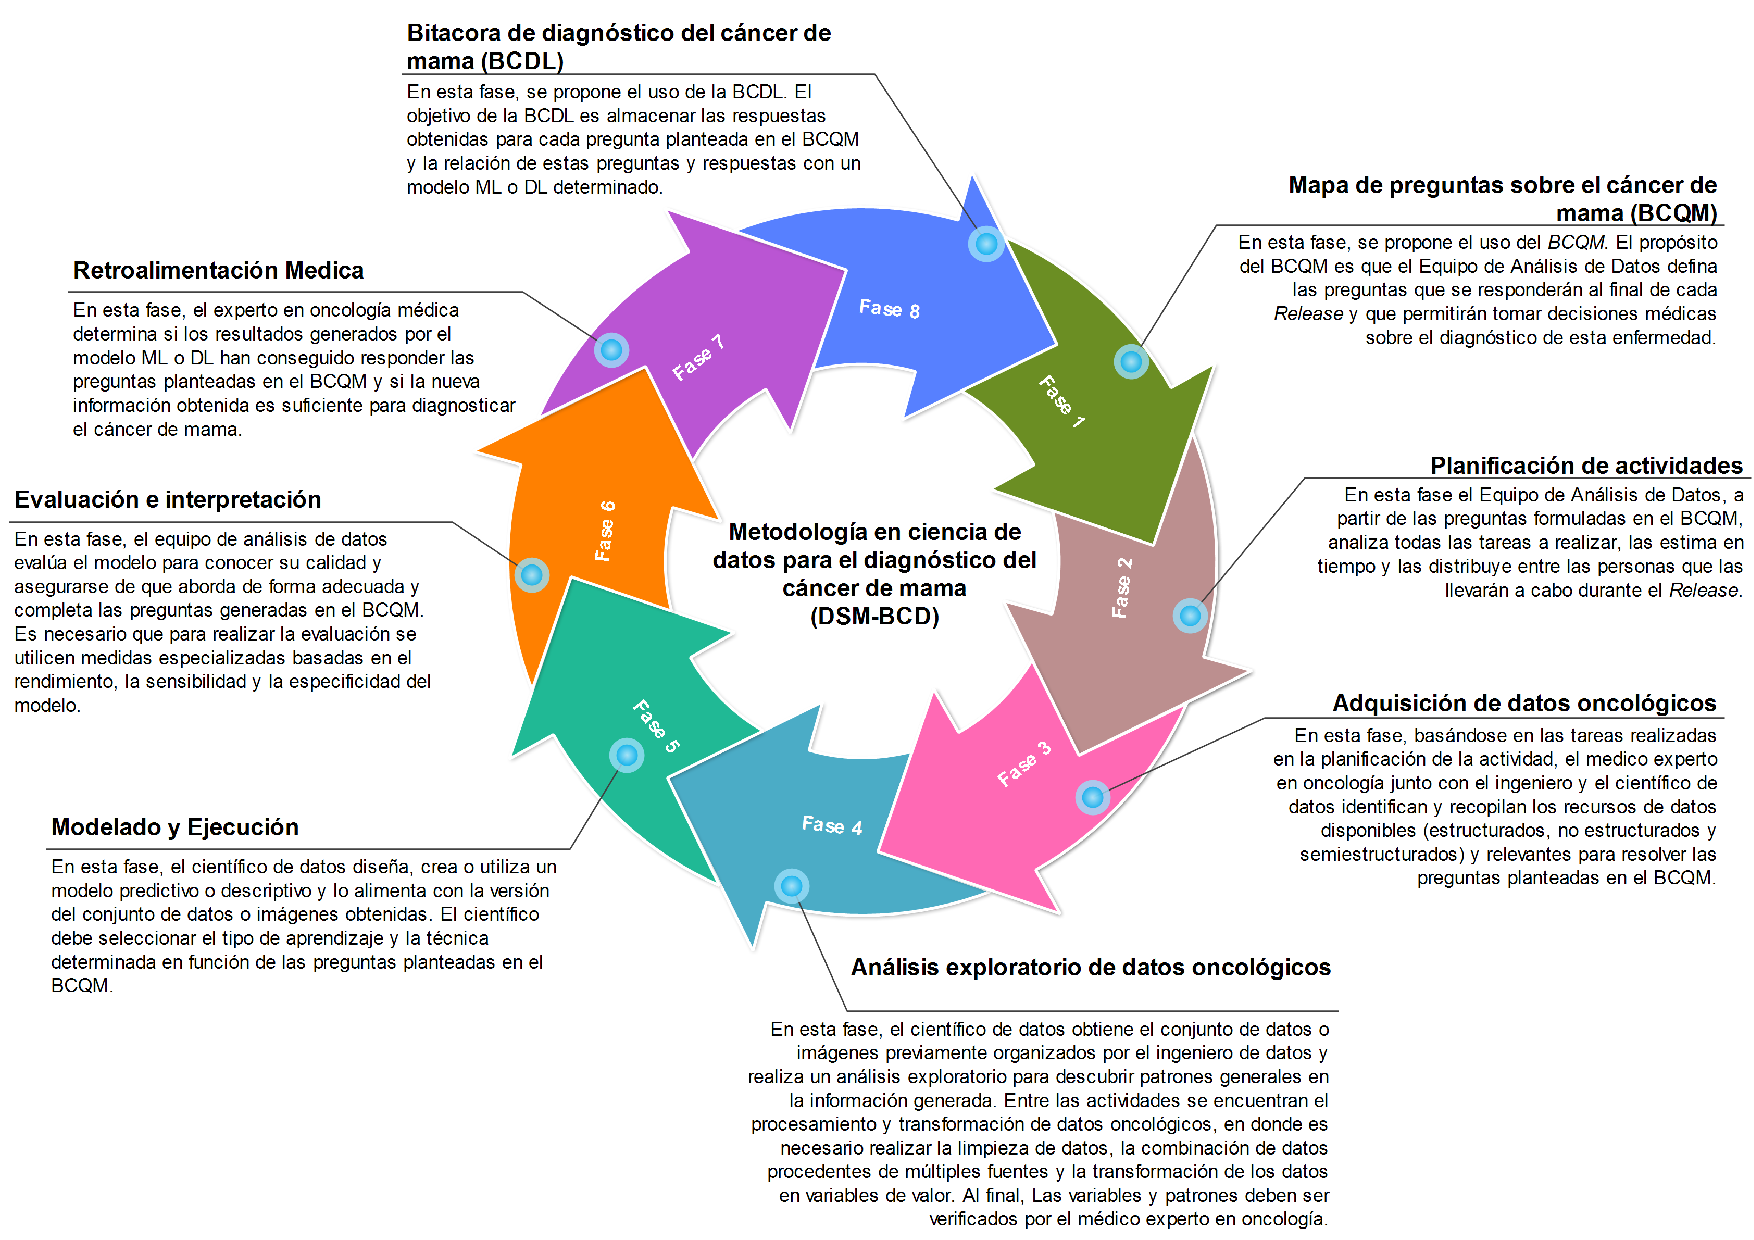
\includegraphics[width=0.87\linewidth]{PROYECTO/imgs/DSM-BCD_SPANISH}
	\end{figure}
\end{frame}

%----------------FRAME---------------------------------------------------
\begin{frame}
	\frametitle{Desarrollo de la Investigación}
	\begin{figure}[h!]
		\centering
		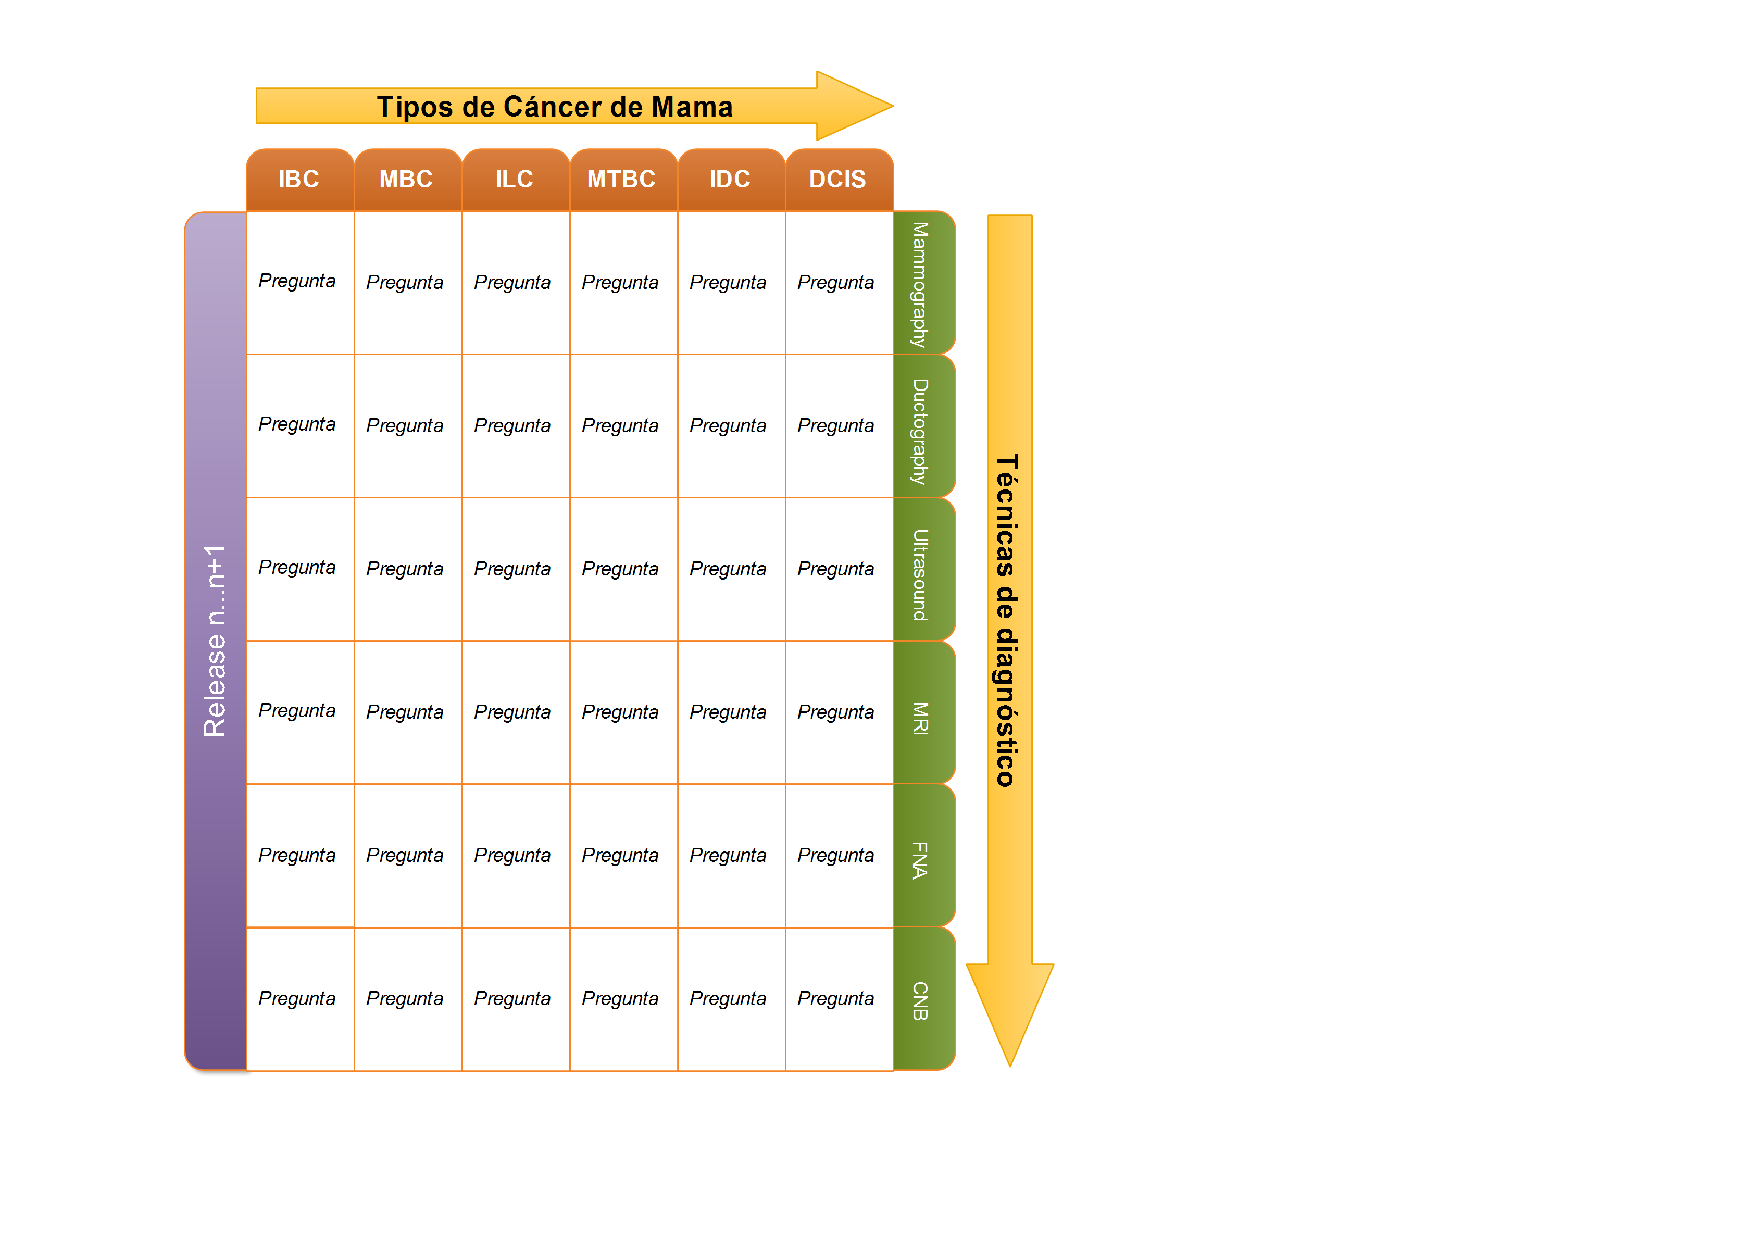
\includegraphics[width=0.56\linewidth]{PROYECTO/imgs/BCQM_SPANISH}
	\end{figure}
\end{frame}



%----------------FRAME----------------------------------------------------
\begin{frame}
	\frametitle{Desarrollo de la Investigación}
	\begin{block}{Fase 1: BCQM}\justifying
	Para este caso de estudio, se plantearon las siguientes preguntas  basados en el atlas del Genoma del Cáncer con la finalidad de catalogar cambios moleculares de importancia biológica responsables de la aparición de cáncer haciendo uso de la secuenciación genómica y la bioinformática.

	\end{block}
	
	\begin{figure}[h!]
		\centering
		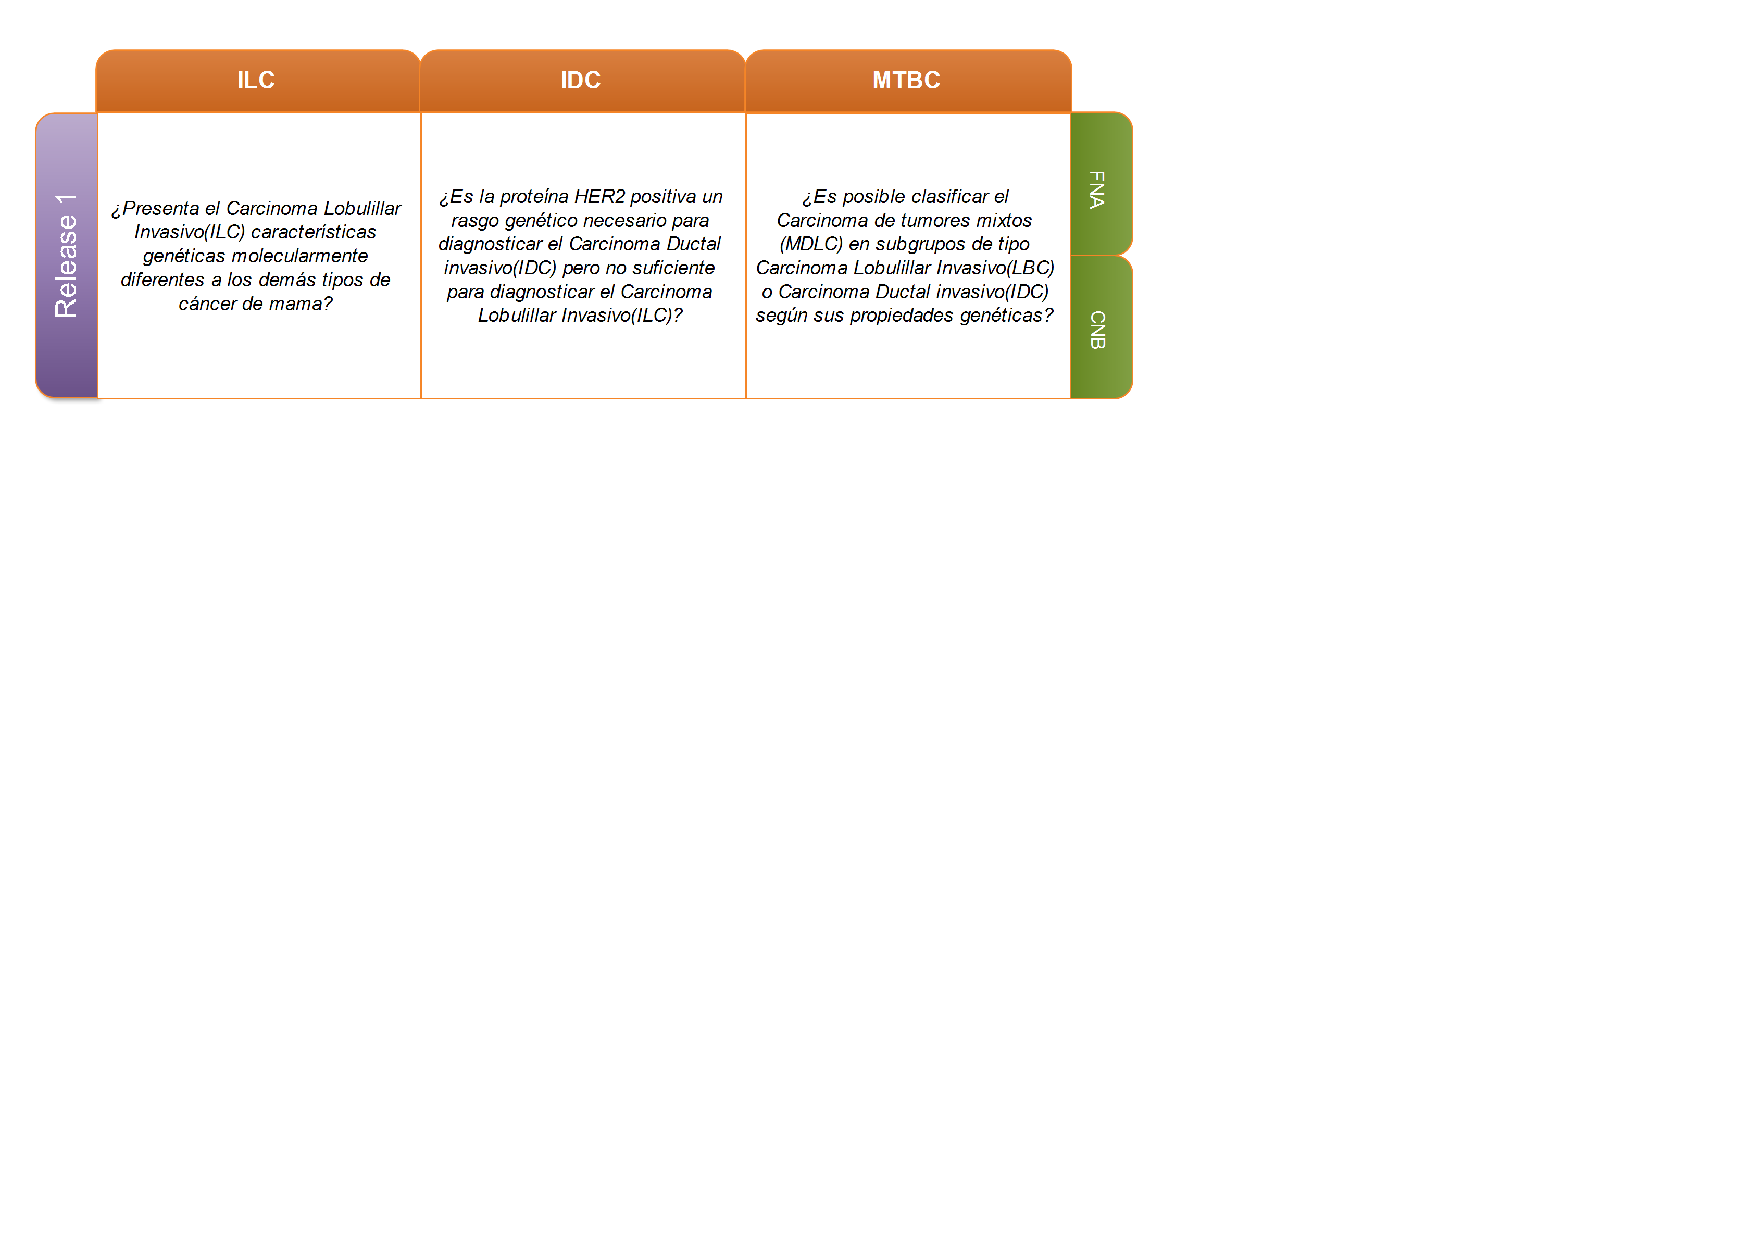
\includegraphics[width=0.93\linewidth]{PROYECTO/imgs/BCQM_TCGA}
	\end{figure}
\end{frame}


%----------------FRAME----------------------------------------------------
\begin{frame}
	\frametitle{Conclusiones}
	\begin{itemize}\justifying
	\item Con respecto a los modelos de Machine Learning utilizados por diversos investigadores para predecir el Cáncer de mama se puede evidenciar que el algoritmo más utilizado es el Support Vector Machines (SVM), pero al realizar la comparación con los resultados obtenidos de la precisión de los métodos de Machine Learning observados anteriormente, el algoritmo Decision Trees es el que mejor resultado tiene, con una exactitud del 100\%, esto quiere decir que clasifico correctamente el total de las muestras. Por lo tanto según la investigación realizada  se concluye que si se va a diagnosticar el Cáncer de mama los modelos más indicados para hacerlo son el Support Vector Machines(SVM) y Decision Trees.
	\end{itemize}
\end{frame}
%----------------FRAME--------------------------------------------------------------
\begin{frame}
	\frametitle{Conclusiones}
	\begin{itemize}\justifying
		\item Según el análisis realizado con base en el diagrama de calor conformado por la correlación de las variables del Data-Set de la Universidad de Wisconsin se puede evidenciar que  las variables \textit{concave\_points\_worst} y \textit{area\_worst} generan información relevante en la realización del diagnóstico de Cáncer de mama debido a  que expresan  una deformidad mayor de los núcleos celulares encontrados en las masas mamarias extraídas por el método de Aspiración con Aguja Fina(FNA).
	\end{itemize}
\end{frame}
%----------------FRAME--------------------------------------------------------------
\begin{frame}
	\frametitle{Aportes Originales}
	\begin{itemize}\justifying
		\item Implementación de una capa de servicios REST basada modelos de Machine Learning para el diagnóstico de Cáncer de mama que podría ser utilizada en diferentes ámbitos en la detección y el diagnóstico de dicho Cáncer.
		
		\item Diseño y Arquitectura de un aplicativo web enfocado en el uso de modelos de Machine Learning aplicados en la rama de la Medicina especializada en Oncología.
	\end{itemize}
\end{frame}

%----------------FRAME--------------------------------------------------------------
\begin{frame}
	\frametitle{Trabajos Futuros}
	\begin{itemize}\justifying
		\item Creación de una aplicación web llamada OncoAnalysisApp la cual permita el diagnóstico de cualquier tipo de Cáncer teniendo como entrada Data-Sets obtenidos por diversos métodos médicos.
		\item Creación de una aplicación que permita el análisis de imágenes y que diagnostique el padecimiento de Cáncer de mama con base a los modelos de Deep-Learning existentes.
		\item Creación de una aplicación que permita crear nuevos Data-Set dinámicamente según parámetros proporcionados por el usuario. 
	\end{itemize}
\end{frame}



%----------------FRAME-------------------------------------------------------------
\begin{frame}
	\frametitle{Bibliografía}	
	\bibliographystyle{unsrt}
	\bibliography{REFERENCIAS/articulos}
\end{frame}


\end{document}